
\documentclass{article}
\usepackage{graphicx}
\title{GRNReasoner 1.0}
\author{Xiaoyu Ge and Jochen Renz}
\begin{document}
\maketitle

\section{Installation}

\begin{itemize}
\item To run the software, java 6 or later version is required.  
\item Download the software package and unzip
\item GRNReasoner.jar is the executable
\item the\textit{ src} folder contains all the source codes
\item the \textit{level} folder contains all the level files. Level files are described in section \ref{input} 
\end{itemize}



\section{Data Format}
\subsection{Input}\label{input}
The algorithm takes a set of MBRs (minimum bounding rectangle) as input. A MBR is represented by its x,y coordinate of the top left corner, width and height. There are two input sources available
\\1. a file containing a list of MBRs specified in the following format:

 In each row, we specify the four values in the order: x, y coordinate, width, and height. Comments should be started with a \#, and \$ indicates the end of the file. More samples files can be found in the $level$ folder
\\\\\# The following is a sample input derived from the level 4 in the poached \\\# eggs episode
\\480 355 16 145
\\514 428 16 72
\\548 428 16 72
\\675 428 16 72
\\713 428 16 72
\\745 355 16 145
\\510 377 72 51 
\\548 412 148 16
\\663 380 72  48
\\588 375 72 37
\\615 301 16 74
\\620 280 140 75
\\480 283 140 72
\\\$ 
\\2. The algorithm can also accept a list of MBRs extracted from the vision module of the Angry Birds basic software 

\subsection{Output}
The algorithm will identify a stable set of GSRs (general solid rectangles) for a given set of MBRs. The output is a list of $configurations$. A $configuration$ of a GSR describes the GSR's unary property and the contacts it holds with other GSRs in form of the GR-n binary relations.  

\subsubsection{Sample Output}
The console will print a list of configurations as a solution in the following format:
\\$\underbrace{MBR\,\,\, uid: \,\,\,11 \,\,\,id: \,\,\,0}_{mbr \,\, key}$ $\underbrace{unary: SL}_{unary\,\, relation}$ $\underbrace{contacted\,\,\, by\,\, [ MBR\,\,\,id:\,\,\,4\,\,\,at\,\,\,Region: S6, touching ]}_{contact \,\,relation}$
\\\\The console will print a list of incomplete configurations as approximation when no solution has been found. A incomplete configuration is a configuration excluding contact relations.
\subsubsection{MBR Key}
\begin{itemize}
\item UID: a MBR is uniquely identified by its uid. UIDs will not be changed during the execution of the algorithm.
\item ID: id indicates the ordering of MBRs during a backtracking procedure. The MBRs will be searched in ascending order by their ids. 
\end{itemize}
\subsubsection{Unary Relations} 
Recalling that we classify GSRs according to how their corners relate to their corresponding MBRs (see Figure \ref{unary}), in the implementation, we use the following five distinctions.  
\begin{figure}[h!]
\centering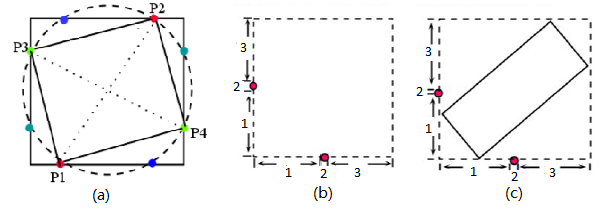
\includegraphics[scale=0.55]{combo1}\caption{(a) Relating MBR and GR (b) The $QCI_{1}$ distinctions (c) A possible instantiation of $M_{1}^{(1,1)}$ using $QCI_{1}$ }
\label{unary} 
\end{figure}

\begin{itemize}
\item SL: slim leaning to left, $M^{(3,3)}$
\item SR: slim leaning to right, $M^{(1,1)}$
\item FL: fat leaning to left, $M^{(1,3)}$
\item FR: fat leaning to right,  $M^{(3,1)}$
\item Regular: regular
\end{itemize}
\subsubsection{Contact Relations}
When two GSRs $m_1$ and $m_2$ touch each other, then they either touch at a point or along a line segment. This contact will be equal to or part of a contact sector (see Figure \ref{sector}) of $m_1$ and a sector of $m_2$.
The contact relation between $m_1$ and $m_2$ indicates which sector of $m_1$ touches which sector of $m_2$.  
\begin{figure}[h!]
\centering\includegraphics[scale=0.35]{sectors.png}\caption{Contact sectors of regular and angular GSRs}
\label{sector}
\end{figure}
E.g. the configuration 
 ${MBR\,\,\, uid:\,11 \,\,\,id:\,0}$ $unary: SL$ $contacted\,\,\, by\,\, [ MBR\,\,\,id:\,\,\,4\,\,\,at\,\,\,Region: S6, touching ]$ means the eMBR with id 0 touches the $S6$ of the eMBR with id 4. You can look up the configuration of  the other eMBR by its id. If the eMBR is regular, then the $S6$ refers to $R6$ otherwise $A6$
\section{Algorithm}
The implementation is based on the algorithm described in the paper with some variance. 

\subsection{Lifting Conflicts}\label{conflict}

Variable ordering is critical to the efficiency of the backtracking. The software will restart backtracking multiple times and the variables are ordered according to the knowledge gained from the previous run. Specifically, the MBRs which are likely to cause branch pruning will be lifted up. 

\begin{figure}[h!]
\centering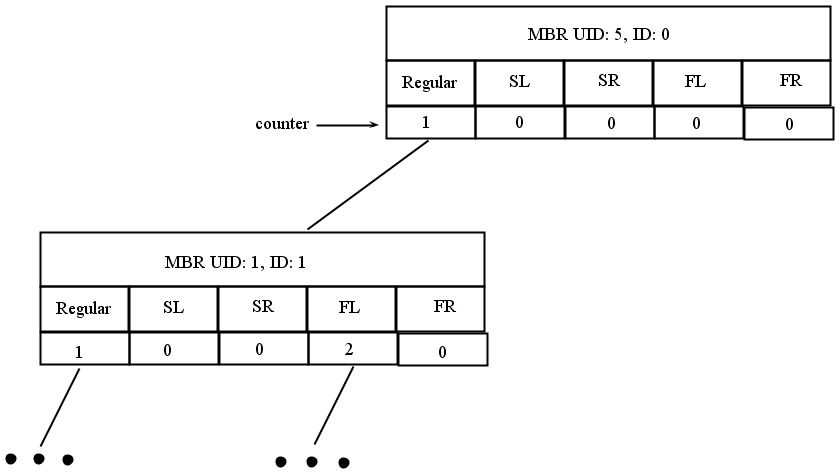
\includegraphics[scale=0.35]{f1.jpg}\caption{Structure of a backtracking tree}
\label{node}
\end{figure}
In a backtracking tree, each MBR is represented as a node see Figure. \ref{node}. We use the aforementioned five unary relations to distinct GSRs . Each of the unary relations is associated with a counter that maintains the number of times a particular eMBR (eMBR is a MBR with one of the five unary relations) reaches the stable status. 

Initially, the MBRs are ordered randomly and the algorithm always expands the MBRs with lower ID. The algorithm expands a node by assigning a unary relation to the MBR which creates an eMBR. Then the algorithm will check if there is any eMBR from the root to the current node that is not stable according the rules of stability (given in the paper). If an eMBR becomes stable, we increase the corresponding counter by one and mark the eMBR as checked (next time the algorithm will skip this eMBR).  Branch pruning happens when there is a unstable eMBR \underline{and} all its neighbors have already been initialized i.e. the eMBR can not be supported by any of its neighbors. The algorithm will backtrack when all the selections of the unary relations result in branch pruning. 
Otherwise the algorithm will continue to expand the next node.


When the time limit of one attempt reaches, the algorithm will re-order the MBRs by evaluating the counters. Specifically, for each of the MBRs, we sum its five counters and if the value is lower than a certain number (say 3000), the MBR will be lifted up and visited earlier in the next backtracking procedure.  



\subsection{Multithreading \& Approximation}
With the help of multi threading, we can run several backtracking procedures simultaneously. There is no communication between those backtracking procedures. Once a solution is found, the algorithm will report it immediately and terminate all the working threads.

If there is no solution, the backtracking will be endless (exponential in time). To deal with this, the algorithm will return an approximation (a list of eMBRs without contact relations) when time limit reaches. The approximation is primarily based on the counters (see section \ref{conflict} ). An eMBR's final counter is the sum of the corresponding counters of all the backtracking procedures. For a particular MBR, the algorithm will choose the eMBR with the highest counter of the five possible eMBRs . For the example shown in Figure \ref{example}, the eMBR with unary relation $FR$ will be chosen because of the highest counter (2700 + 6000 = 8700) 

Besides, the overlapping areas of the MBRs are also considered for approximation. (see ApproximateSolution.java).   	

\begin{figure}[h!]
\centering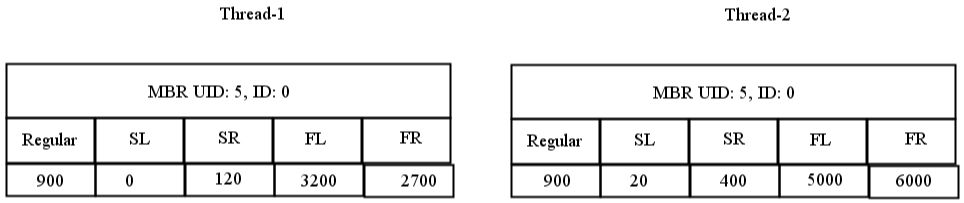
\includegraphics[scale=0.35]{f2.jpg}\caption{Approximate the eMBR of the MBR with UID5 }
\label{example}
\end{figure}




\section{Run the Software}
\begin{itemize}
\item Using file input: java -jar GRNReasoner.jar $[option]^*$ [file directory]
\item Using vision input: java -jar GRNReasoner.jar $[option]^*$ vision
\end{itemize}
You can specify the following parameters in the option field (the option field is optional):
\begin{itemize}
\item $-gap\,\,[num]$: if the space between two disjoint MBRs is smaller than the specified value, then the space will not be considered as a gap by the algorithm. i.e. the algorithm will consider the two MBRs as tangential instead.
\item $-t\,\,[num]$: the number of working threads allowed 
\item $-attempt\,\,[num]$: the number of attempts. The backtracking will be restarted per attempt
\item $-time\,\,[num]$: the number of time units (in seconds) per attempt. An attempt of the backtracking will be terminated when the time limit reaches
\end{itemize}
If no parameters are specified, the algorithm will use the default values. E.g. java -jar GRNReasoner.jar level/l4 is equivalent to java -jar GRNReasoner.jar -gap 10 -t 1 -attempt 5 -time 4 level/l4
\begin{figure}[h!]
\centering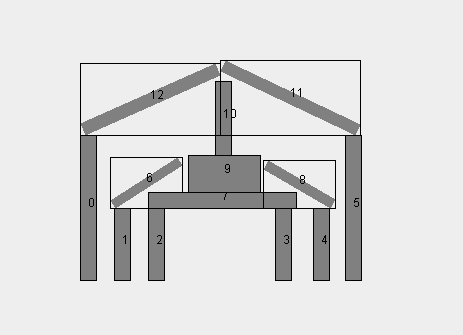
\includegraphics[scale=0.35]{l4vo.png}\caption{The output of java -jar GRNReasoner.jar level/l4 }
\label{example}
\end{figure}
Note, you need to open a chrome angry birds window when run with the vision input.


\section{Run with Chrome Angry Birds} 
You can use the software along with the vision module of the Angry Birds basic software to estimate possible stable configurations over a set of MBRs extracted from a screenshot. The result depends on the accuracy of the MBR detection. 

The following is a java code fragment to show how to apply the algorithm to the angry birds software.
\\
\\//Get the screenshot
\\new ActionRobot();
\\BufferedImage screenshot = ActionRobot.doScreenShot();
\\
\\//Segmentation
\\Vision vision = new Vision(screenshot);
\\\\//Get MBRs and add it to a list
\\ LinkedList$<$Rectangle$>$ worldInVision = new LinkedList$<$Rectangle$>$(); 
\\worldInVision.addAll(vision.findStones());
\\worldInVision.addAll(vision.findWood());
\\ worldInVision.addAll(vision.findIce());
\\worldInVision.addAll(vision.findPigs());
\\
\\//Pre-process and show all the MBRs  
\\WorldinVision wiv = new WorldinVision();
\\wiv.buildWorld(worldInVision); 
\\wiv.showWorldinVision(null , null ,null);
\\
\\//Initialize the algorithm and run it	  
\\MultiThreadReasoner multiReasoner = new MultiThreadReasoner(wiv, threads ,attempt, time); 
\\multiReasoner.run();





\end{document}

